\chapter{Graphs}

\pgfplotsset{width=1\columnwidth,compat=1.9}

\begin{tikzpicture}
\begin{axis}
\addplot[color=red]{exp(x)};
\end{axis}
\end{tikzpicture}

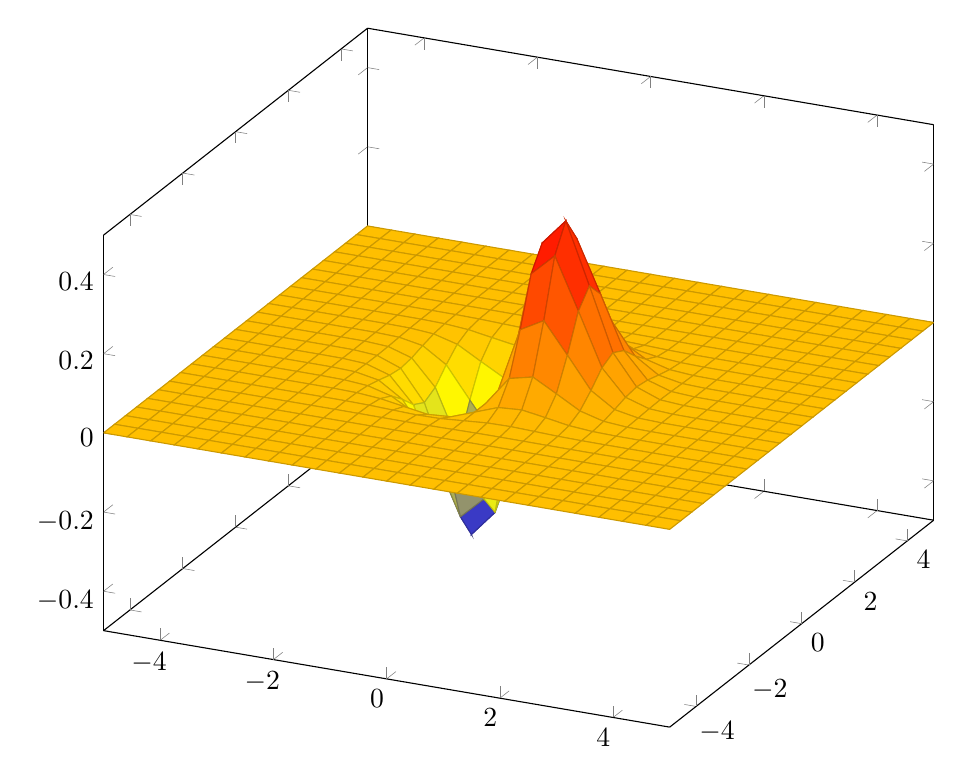
\begin{tikzpicture}
\begin{axis}
\addplot3[surf,]
{exp(-x^2-y^2)*x};
\end{axis}
\end{tikzpicture}

\hskip 10pt

\begin{tikzpicture}
\begin{axis}[
axis lines = left,
xlabel = $x$,
ylabel = {$f(x)$},
]
%Below the red parabola is defined
\addplot [
domain=-10:10, 
samples=100, 
color=red,
]
{x^2 - 2*x - 1};
\addlegendentry{$x^2 - 2x - 1$}
%Here the blue parabloa is defined
\addplot [
domain=-10:10, 
samples=100, 
color=blue,
]
{x^2 + 2*x + 1};
\addlegendentry{$x^2 + 2x + 1$}

\end{axis}
\end{tikzpicture}

